\documentclass[a4paper,11pt]{article}
\usepackage{t1enc}
\usepackage[space]{grffile}
\usepackage[round, longnamesfirst]{natbib}  % Bindet den natbib-standard fuer das Zitieren ein
\usepackage{epsfig}
\usepackage{chngcntr}
\usepackage[latin1]{inputenc}   % Ermoeglicht Sonderzeichen direkt einzugeben
\usepackage[T1]{fontenc}        % Garantiert saubere Worttrennung bei Umlauten etc.
\usepackage{color}              % Farbpaket
\usepackage{amsmath,amsfonts,amssymb}   % ermoeglicht mathematische Sonderzeichen
\usepackage[english]{babel}     %
\usepackage{ae}                 %
%\usepackage{graphicx,subfigure}           % Ermoeglicht das Einbinden von Bildern in allen Formaten
\usepackage{graphicx}
\usepackage{longtable}          % zum erstellen von Tabellen ber mehrere Seiten
\usepackage{multirow}           % zum Verbinden von Zeilen innerhalb einer Tabelle
%\usepackage{pictexwd}           % PicTex, ein Graphikpaket
\usepackage{pst-all, multido}   % psTricks, ein Graphikpaket
\usepackage{url}
\usepackage[doublespacing]{setspace}
\usepackage{booktabs,caption,fixltx2e,array,dcolumn}
\usepackage{parskip}
\usepackage{etoolbox}
\usepackage{tabularx}
\usepackage{caption}
\usepackage{subcaption}
%\usepackage{morefloats}
\usepackage[section]{placeins} % Mit FloatBarrier kann verhindert werden, dass Float in der nächsten Section angezeigt werden
\usepackage[bottom]{footmisc} % Fußnoten werden ganz unten angezeigt
\setcitestyle{authoryear, open={((},close={))}}

\newcolumntype{L}[1]{>{\raggedright\arraybackslash}p{#1}} % linksbündig mit Breitenangabe
\newcolumntype{C}[1]{>{\centering\arraybackslash}p{#1}} % zentriert mit Breitenangabe
\newcolumntype{R}[1]{>{\raggedleft\arraybackslash}p{#1}} % rechtsbündig mit Breitenangabe

\makeatletter
\interfootnotelinepenalty 10000
\patchcmd{\Ginclude@eps}{"#1"}{#1}{}{}
\makeatother

\makeatletter
\newcommand\tageq{%
  \ifmeasuring@\else
    \refstepcounter{equation}%
  \fi
  \tag{\theequation}%
}
\makeatother

\newcommand\fnote[1]{\captionsetup{font=tiny}\caption*{#1}}

%\parindent 0cm
%\renewcommand{\baselinestretch}{1}

\renewcommand{\bibnumfmt}[1]{#1.}
\bibpunct{(}{)}{;}{a}{,}{,}

%%%%%%%%%%%%%%%%%%%%%%%%%%%%%%%%%%%%%%%%%%%%%%%%%%%%%%%%%%%%%%%%%%%%%%%%%%%%%%%%%%%%%%%%%%%%%%%%%%%%%%%%%%%%%%%%%%%%%%%%%%%%%%%%%%%%


% ________________ EINRICHTEN DES DOKUMENTS ______________________%

%\bibliographystyle{plainnat}    % legt den Stil fuer das Inhaltsverzeichnis fest

\oddsidemargin 0.0in \evensidemargin 0.0in \textwidth 15.5cm \topmargin -0.8in \textheight 24.5cm
\setlength{\parskip}{0pt}
\setlength{\parindent}{10pt}
\renewcommand{\baselinestretch}{1}


\setlength{\intextsep}{0.5cm} % Legt den Abstand zwischen Gleitobjekten und dem darüber und darunter angeordneten Fließtext fest.

%\oddsidemargin 0.1in \evensidemargin 0.1in \textwidth 15.5cm \topmargin -0.4in \textheight 24.5cm
%\parindent 0cm      % legt die Seitenraender fest

\pagestyle{plain}          % leere Kopfzeile, Seitennummer in der Mitte der Fusszeile

\newcommand{\bs}{\boldsymbol}  % shortcut zur Erzeugung von fetten Sympolen in der Mathe-Umgebung

%\renewcommand{\baselinestretch}{1.25}
% 1,5 -facher Zeilenabstand (Standard ist 1,2-facher Zeilenabstand, also 1,2*1,25 = 1,5

\begin{document}

\pagenumbering{roman}   % roemische Zahlen zur Seitennumerierung


%%%%%%%%%%%%%%%%%%%%%%%%%%%%%%%%%%%%%%%%%%%%%%%%%%%%%%%%%%%%%%%%%%%%%%%%%%%%%%%%%%%%%%%%%%%%%%%%%%%%%%%%%%%%%%%%%%%%%%%%%%%%%%%%%%%%%%%5


\begin{titlepage}       % Umgebung fuer Titelseite, frei gestaltbar

\thispagestyle{empty}   % keine Numerierung auf Titelseite

\begin{center}

\includegraphics[width=13cm]{Bild.png}
\end{center}

\begin{center}

\vspace*{1.5cm}
{\bf  \Large Assignment \#2: Implicit Finite Difference Methods} \\
\vspace*{2cm} 
\textbf{B473 Numerical Methods in Finance}
\\
Prof. Dr.-Ing. Rainer Sch\"obel
\\
\vspace*{0.5cm} 
Winter Term 2016-2017\\
\end{center}

\vfill
\begin{flushright}
    \emph{Konstantin Smirnov}\\
    \textit{Student-ID: 3980253}\\
     \textit{ Economics and Finance}\\
 T\"ubingen, \today
  




\end{flushright}



% 
% \begin{center}
% $ $			% oeffnet und schliesst eine Matheumgebung (Trick, um den Titel nach unten zu rutschen
% \vspace{4cm}
% 
% {\LARGE TITEL}
% \vskip 4cm
% 
% Diese Seite ist frei gestaltbar
% \end{center}

\end{titlepage}

\newpage                % erzwingt an dieser Stelle einen Seitenumbruch

\listoffigures
\newpage


\tableofcontents

\newpage
\pagenumbering{arabic}      % Seitenzahlen wieder arabisch numerieren
\setcounter{page}{1}        % Ruecksetzen des Seitenzahlzaehlers auf 1
\section{Introduction}
This paper examines how the Implicit and the Crank-Nicolson Finite Difference Method is used to solve numerically for the Black-Scholes Merton partial differential equation (PDE) with the focus on an European Put. Generally speaking the Finite-Difference methods uses a Taylor series expansions in order to approximate the partial derivatives terms of the PDE (Brandimarte, 2006). The implicit scheme proceeds forward in time to solve the PDE, while the Crank-Nicolson Method can be described as a combination of the implicit and explicit scheme method.

Also both methods are extended with a Richardson extrapolation to increase accuracy. In the end of this paper it will be analysed which of the the four methods is the most efficient regarding accuracy and computational effort.
\section{Implicit Finite Difference Method for an European Put}
\subsection{Theoretical Framework}
The Black-Scholes-Merton-PDE is defined as:
\begin{equation}
\frac{1}{2}\eta^2 S^2 F_{SS}(S,T) + (r - q) SF_{S}(S,t) - rF(S,t) + F_{t}(S,T) = 0.
\label{PDE1}
\end{equation}
where $\eta^2$ is the volatility, S is the stock price, r is the risk-free rate, q is the continuous payed dividend and F(S,T) is the payoff function of the option depended of the stock price S and time to maturity T. Since we are interested in the values of an European Put option, we use the following payoff function (Hirsa, 2013): 
\begin{equation}
F(S,T)= max(E-S(T),0)
\label{EuroPut}
\end{equation}
where S is the stock price at time-to-maturity T and E as the strike price of the option.
\subsubsection{Defining a Grid}
To solve the PDE (\ref{PDE1}) with the Finite Difference method, we have to set up a grid first by discretizing our input variables S and T as it was the case in the explicit scheme assignment.
Hence, we define our input variables as
\begin{equation*}
x=S=ih \text{, where } i \in [0,M]
\end{equation*}
and
\begin{equation*}
\tau = T-t=nk \text{, where }  n \in [0,N]
\end{equation*}
where i and n are index numbers, and h and k are step sizes with respect to the stock price and time.
Hence one can define the rectangular grid as
\begin{equation*}
x \in [0,x_{max}] \text{, with } x_{max}= M \cdot h
\end{equation*}
and
\begin{equation*}
\tau \in [0,T] \text{, with } T = N \cdot k
\end{equation*}
Discretizing the PDE of the European Put at the points x and $\tau$ leads to the following equation:
\begin{equation}
a(i,n)u_{xx}(i,n)+b(i,n)u_{x}(i,n)+c(i,n)u(i,n)-u_{\tau}(i,n)=0
\label{PDE2}
\end{equation} 
with
\begin{eqnarray*}
a(i,n)&=&\frac{1}{2}\eta^2 i^2 h^2\\
b(i,n)&=&(r-q)ih\\
c(i,n)&=&-r
\end{eqnarray*}
\subsubsection{Difference Approximation of the Implicit Scheme}
In order to approximate the discretized PDE (\ref{PDE2}) with the implicit scheme, we use following Taylor series expansions in order to approximate the partial derivatives (Fusai and Roncoroni, 2008).
\\
The central approximation of the gamma term $\Gamma$:
\begin{equation}
[U_{xx}]^{n+1}_{i}= \frac{1}{h^2}(U_{i+1}^{n+1} - 2 U_{i}^{n+1} + U_{i-1}^{n+1}) + \mathcal{O}(h^2)
\label{Pgamma1}
\end{equation}
The central approximation of the delta term $\Delta$:
\begin{equation}
[U_{x}]^{n+1}_{i}= \frac{1}{2h}(U_{i+1}^{n+1} - U_{i-1}^{n+1}) + \mathcal{O}(h^2)
\label{central1}
\end{equation}
the forward approximation for the theta term $\Theta$:
\begin{equation}
[U_{\tau}]^{n+1}_{i}= \frac{1}{k}(U_{i}^{n+1} - U_{i}^n{n}) + \mathcal{O}(k)
\label{Ptheta1}
\end{equation}
Plugging these approximations (\ref{Pgamma1}),(\ref{central1}), and (\ref{Ptheta1}) into our discretized PDE (\ref{PDE2}), we get following equation:
\begin{equation}
\frac{a}{h^2}(U_{i+1}^{n+1} - 2 U_{i}^{n+1} + U_{i-1}^{n+1}) + \frac{b}{2h}(U_{i+1}^{n+1} - U_{i-1}^{n+1}) + c U^{n+1}_{i} - \frac{1}{k}(U_{i}^{n+1} - U_{i}^n{n}) = 0
\label{rearr}
\end{equation}
%Note that compared to (3), the approximation of \textit{u(i,n)} does not have to be taken into account because the error of this adjustment tends to zero with increasing grid points (Brandimarte, 2006).\\
Rearranging (\ref{rearr}) in order to solve for $U_{i}^{n}$ leads to the implicit solution for the grid points at $x=ih$ and $\tau = nk$ for all $i \in [1,M-1]$ and $n \in [0,N-1]$ :\footnote{These approximations are still independent of the time index n.}
\begin{equation}
d_1(i,n+1)U_{i-1}^{n+1} + d_2(i,n+1)U_{i}^{n+1} + d_3(i,n+1)U_{i+1}^{+1n}  = d_4(i,n+1)
\label{PDE3}
\end{equation}
with
\begin{align*}
& d_1(i,n+1) = -a\frac{k}{h^2}+b\frac{k}{2h}=-\frac{1}{2}\eta^2 i^2 k + \frac{1}{2}(r-q)ik \\
& d_2(i,n+1) = a\frac{2k}{h^2} -ck +1= \eta^2 i^2 k+(r-q)k +1\\
& d_3(i,n+1) = -a\frac{k}{h^2}-b\frac{k}{2h}=-\frac{1}{2}\eta^2 i^2 k - \frac{1}{2}(r-q)ik \\
& d_4(i,n+1) = U_{i}^{n} \\\\
\end{align*}
At this point it should be made clear that the discretized PDE can be described as recursive algorithm consisting of linear equations. Only the RHS is known while on the LHS we have M unknowns at each time step n. Hence methods like the Gaussian elimination can be used to solve for the system. This will be discussed in section \ref{Chapter:MatrixandSolution} in more detail. 
\subsubsection{Truncation Error}
In order to derive the truncation error of the fully implicit scheme, we need a closer look at the Taylor series expansion around $x=ih$ and $\tau=(n+1)k$ (Sturm, 2017):
\begin{align*}
u(x \pm h,\tau)&=u(x,\tau) \pm hu_x + \frac{1}{2} h^2 u_{xx}  \pm \frac{1}{6} h^3 u_{xxx} + \frac{1}{24} h^4 u_{xxxx} \pm \ldots \\
u(x,\tau - k)&=u(x,\tau) - k u_{\tau} + \frac{1}{2} k^2 u_{\tau \tau} - \ldots
\end{align*}
Plugging them into the rearranged discretized PDE in (\ref{rearr}) leads to:
\begin{align*}
a u_{xx} + \frac{a}{12}h^2 u_{xxxx}+bu_x + b \frac{h^2}{6} u_{xxx}+cu-u_{\tau}+\frac{1}{2}k u_{\tau \tau} + O(h^4, k^2)=0 \; .
\end{align*}
Since  (\ref{PDE2}) holds we get following truncation error for the implicit scheme:
\begin{align*}
T^{Imp}(i,n)&= h^2 \left(\frac{a}{12} u_{xxxx} + \frac{b}{6} u_{xxx} \right) + k\left( \frac{1}{2} u_{\tau \tau} \right) + O(h^4, k^2) \\
T^{Imp}(i,n)&=O(h^2, k) \; .
\end{align*}
\subsubsection{Boundary Conditions}
One of the major aspects of the finite difference method are the boundary conditions. It should be made clear that in the implicit scheme boundaries have to be also established for the LHS and RHS of equation system (\ref{PDE3}).

The terminal condition is simply defined as the payoff function of the European Put because the value at maturity is known:
\begin{equation*}
U_{i}^{0} = max(E - ih, 0)
\label{b1}
\end{equation*}
\\
For the left-hand boundary we use a \textit{Dirichlet} boundary condition, which in our case is described as the discounted exercise price $U^{n+1}_0 = Ee^{-r(n+1)k}$.\\ 
For $i=0$, we hence get: 
\begin{gather*}
	d_2U^{n+1}_1 + d_3U^{n+1}_2 = d_4^* \text{ with } d_4^*(1,n+1) = d_4(1,n+1) - d_1(1,n+1)U^{n+1}_0. \label{eq:implicit_left}
\end{gather*}
For the right-side boundary, we will use a \text{von Neumann} boundary where we assume that the first derivative of the value at the grid point $(n+1,M)$ with respect to stock price is zero.

Economically speaking this means that if the stock price varies, the value of the option remains constant. Using the second central difference approximation (\ref{central1}) at the right-side border M with respect to our \textit{von-Neumann} boundary condition leads to:
\begin{gather*}
	\left(U_{x}\right)^{n+1}_M \approx \frac{1}{2h}\left(U^{n+1}_{M+1}-U^{n+1}_{M-1}\right) \overset{!}{=}0. \label{eq:derivative}
\end{gather*}
As already discussed in the explicit scheme framework, we can get rid of the 'ghost points' $U^{n+1}_{M+1}$ because we assume that the boundary point next to our boundary point M+1 should also have approximately a slope of 0.\\
Hence we get:
\begin{gather*}
	d_1^*U^{n+1}_{M-1}+d_2^*U^{n+1}_{M} = d_4 \text{ with } d_1^*(M,n+1) = d_1(M,n+1)+d_3(M,n+1). \label{eq:implicit_right}
\end{gather*}
\subsubsection{Matrix Notation and Solution of the System}
\label{Chapter:MatrixandSolution}
In order to solve for the linear equation system of of the discretized PDE with respect to the boundaries, we use matrix notation in order to solve for the system.\\
Since we have $M$ linear equations with $M$ unknowns, we hence get:\footnote{$d_1^*$ as in (\ref{eq:implicit_right})}
\begin{gather*}
\underbrace{\begin{bmatrix} 
		d_2(1) & d_3(1) & & & \\ 
		d_1(2) & d_2(2) & d_3(2) & & \\ 
		& & \ddots & & & \\ 
		& & d_1(M-1) & d_2(M-1) & d_3(M-1)  \\
		& & & d_1^*(M) & d_2(M) 
	\end{bmatrix}}_{\mathbf{A}} \cdot
	\underbrace{\begin{bmatrix} 
		U^{n+1}_1 \\ 
		U^{n+1}_2 \\ 
		\vdots \\ 
		U^{n+1}_{M-1}  \\
		U^{n+1}_{M} 
	\end{bmatrix}}_{U^{n+1}} = 
	\underbrace{\begin{bmatrix} 
		d_4(1) - d_1(1)U^{n+1}_0 \\ 
		d_4(2) \\ 
		\vdots \\ 
		d_4(M-1)  \\
		d_4(M)
	\end{bmatrix}}_{d_4}
\end{gather*}
As already discussed this system can be solved by using Gaussian elimination. However, as the \textbf{A} is of tridiagonal structure, it is more efficient to use a LR-decomposition to solve for the system (Brandimarte, 2006).\\ 
The system is described as:
\begin{gather*}
\underbrace{\mathbf{A}}_{MxN}\underbrace{u}_{Mx1} = \underbrace{d}_{Mx1}
\end{gather*}
In the LR-Decomposition we first transform the A matrix into two matrices, where L is a lower triangular matrix and R is an upper triangular matrix:
\begin{gather*}
(\textbf{L R})u=d
\end{gather*}
This can be rearranged to:
\begin{gather*}
\textbf{L}\underbrace{(\textbf{R}u)}_{y}=d
\end{gather*}
Now the system can be solved with respect to:
\begin{gather*}
\textbf{L}y=d \\
\textbf{R}u=d \\
\end{gather*}
which is far more efficient because the number of operations with the LR-decomposition method only increases linearly compared to Gaussian elimination.
\subsection{Discussion of Results}
In our computations following parameters are used:\\
\begin{align*}
& S_{min} = 200 \qquad\qquad M=120\\
& S_{max} = 1200 \qquad\quad N=100\\
& E = 200\\ 
& T-t = 1.00\\ 		 
& r = 0.04\\
& q = 0.06\\
& \eta=0.25 \\
\end{align*}
\begin{figure}[!h]
\begin{subfigure}[c]{0.5\textwidth}
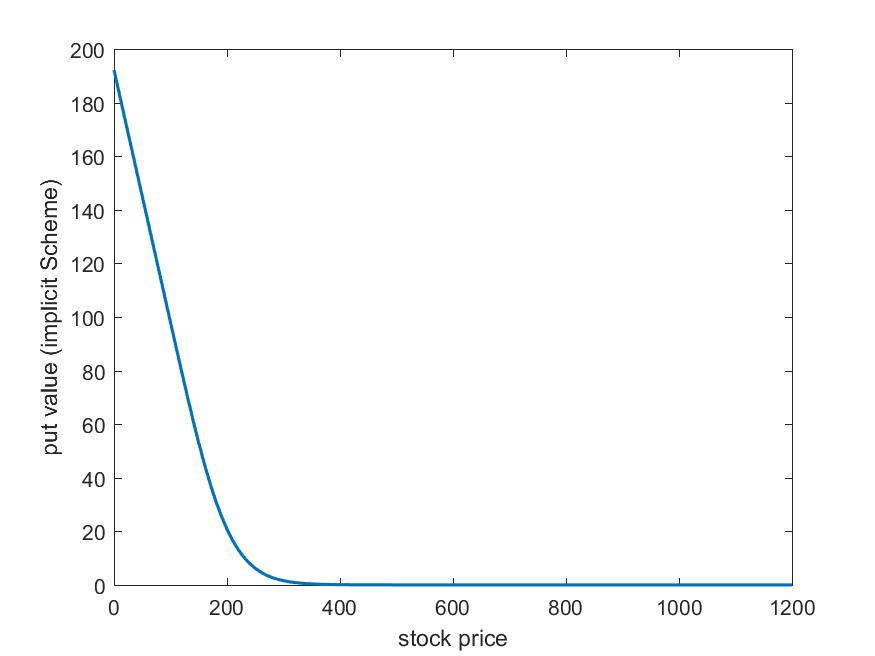
\includegraphics[width=8.5cm]{ImplicitPut.jpeg}
\subcaption*{Implicit Scheme}
\end{subfigure}
\begin{subfigure}[c]{0.5\textwidth}
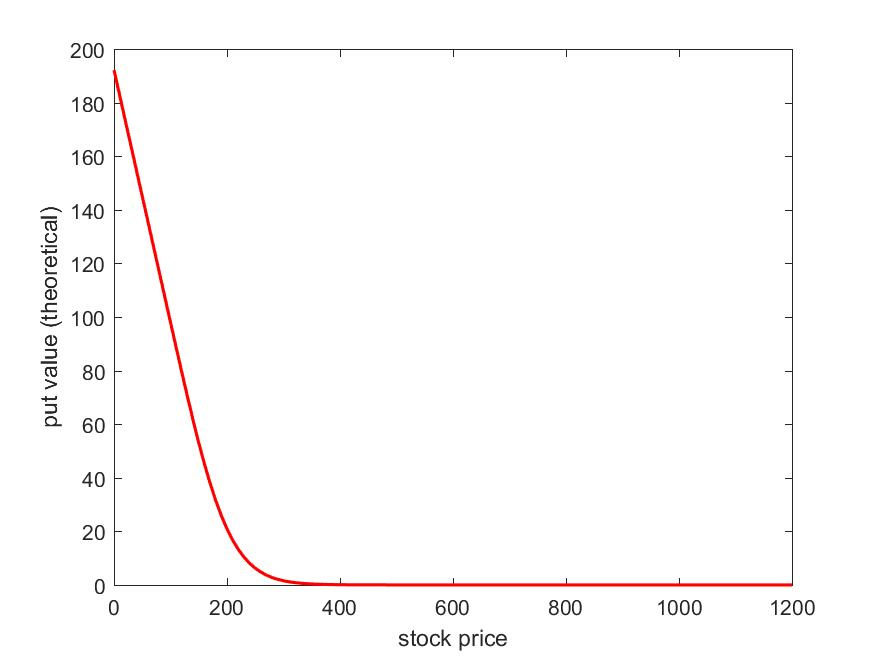
\includegraphics[width=8.5cm]{TheoEuroPut.jpeg}
\subcaption*{Theoretical}
\end{subfigure}
\caption{European Put value for different S - Implicit Scheme vs. Theoretical}
\label{payoffPutImp}
\end{figure}\\
The left plot of figure \ref{payoffPutImp} shows the value of an European Put for different stock price levels with a time to maturity of 1 with respect to the other parameters and step-sizes calculated with the implicit scheme algorithm. The right plot depicts the theoretical computation (benchmark). As it can clearly be seen, the values only diverge minimally in those illustrations. For a stock price of 200 we get an explicit finite difference value of 20.7655 and for the closed-form solution we get a value of 20.8886.

In order to get a closer examination on the divergence of the implicit scheme method, the approximated values will directly be compared with the theoretical benchmark values. We define this divergence from now on as our error term:
\begin{equation*}
Error= u_0(M,N) - BSMP
\end{equation*}
where $u_0$ and the BSMP are vectors which contain all calculated Put values solved with the explicit scheme or respectively with the closed form solution.

These errors are illustrated in figure \ref{2DErrorPutImp} for different levels of S (from 0 to 1200) with a time to maturity of 1. As it can be seen the biggest deviation of 0.1231 can be found when the option is at-the-money. As it was already described in the explicit scheme assignment, at this points it is not possible to take the derivatives due to discontinuity. Hence we get relatively poor approximations at these grid points.

As we have seen in the derivations in the theoretical part, the error vanishes with a speed of $h^2$ at each following approximation in space dimension.
\begin{figure}[!h]
\centering
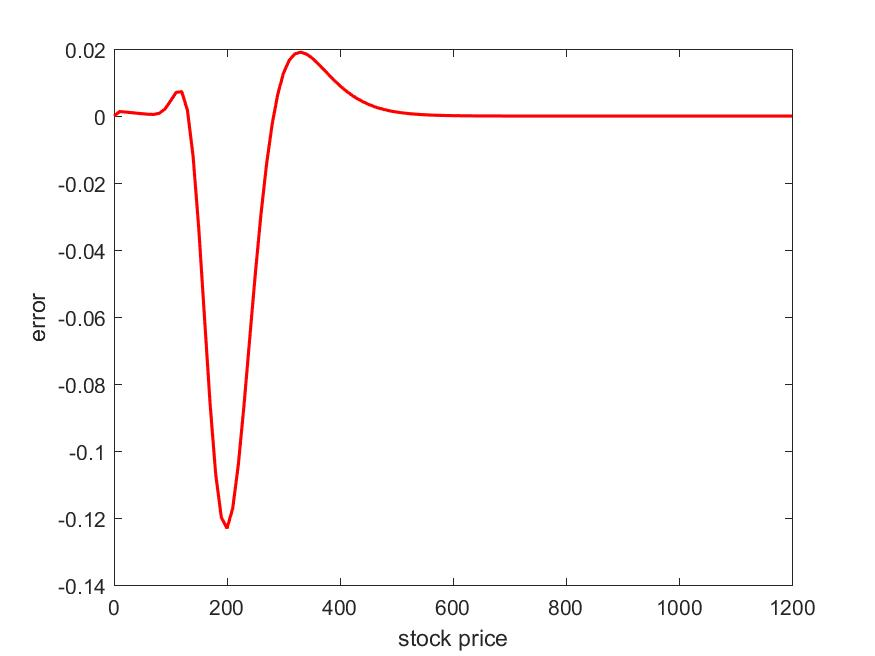
\includegraphics[width=10cm]{2D_Implicit.jpeg}
\caption{Implicit Scheme - Error vs. Stock Price}
\label{2DErrorPutImp}
\end{figure}
\begin{figure}[h!]
\centering
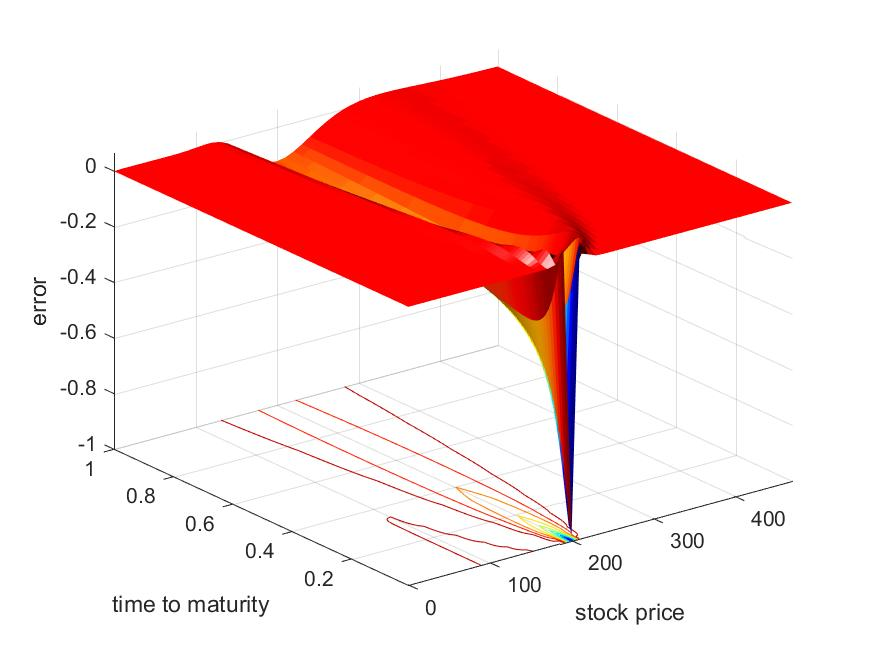
\includegraphics[width=10cm]{3D_Implicit.jpeg}
\caption{Implicit Scheme - Error vs. Stock Price vs. Time to Maturity}
\label{3DErrorPutImp}
\end{figure}

In figure \ref{3DErrorPutImp} the 3D errors for increasing time to maturity are illustrated. Also here we can clearly see that the biggest deviations can be found when the option is at the money for the same reason as just discussed.

Also relatively big deviations can be observed when the option has a short time-to-maturity level of n. The upside probability for options with a very short time to maturity are misapproximated due to the same reason as we discussed in the explicit scheme in the former assignment. The maximum absolute deviation which can be found in this analysis is 0.9740.

The error itself vanishes with the speed of the step-size \textit{k} and takes longer to vanish compared to the truncational error of the stock price approximations $h^2$.

\subsection{Technical Implementation}
The first part of the the main script \textit{$Task71\_73.m$} contains all necessary computations and plots to compute the price of an European Put for different stock prices. The script basically calls the function $Implicit.m$ which consists of the main algorithm for the implicit scheme.

To preserve the outline only the step-size parameters \textit{i} and \textit{n} serve as input variables. To change other input parameters one can adjust it in the algorithm function $Explicit\_EuroPut.m$ itself.

The algorithm basically follows all steps which I described in the theoretical framework of this chapter. The idea of the algorithm is to define all time independent variables out of the main for-loop to improve efficiency. First we discretize our framework with respect to\textit{ d1,d2 and d3} and implement the time independent boundary, as it was discussed in the theoretical part of this chapter.

In the next steps we start with the LR decomposition. Note here that we decided to use the self-written algorithm of the LR-decomposition instead of the implemented \textit{Matlab} function \textit{lu}. As we experienced the self-written algorithm is far more efficient than the \textit{lu} function regarding computational time. As the A matrix is of triangular structure it is more efficient to adjust the LR-decomposition to this special case which can probably not be considered by the implemented \textit{Matlab} function \textit{lu}.

First we decompose the A-Matrix with a loop into a lower and an upper triangular matrix LR. After that we start with our main for-loop which counts for all time steps \textit{n} in order to solve the equation system at each time step. First the time depended boundaries have to be implemented into the main-loop as it was described in the theoretical part. After that we first solve the system Ly = d with a further for-loop, before we finally continue to solve the system for Ru=y. These values are stored in a \textit{u0} which is the final European Put price for the given S at the time to maturity level of 1. To compute the 3D-errors we subtract the theoretical Put price, which is again calculated with an self-written functions \textit{BSMP.m and N.m} at this certain time step, and are stored in an own \textit{ERROR}-matrix. After the main-loop we compute the 2D-error by subtracting the theoretical price from the last u0 vector. Furthermore we search for absolute maximum errors of the 2D error and 3D error cases.

Taking everything into account,  we output the last \textit{u0\_Implicit} vector, the errors \textit{ERROR\_2D\_Implicit} and the \textit{ERROR\_3D\_Implicit}, as well as the maximum errors \textit{ME\_Implicit\_2D} and \textit{ME\_Implicit\_3D}, for the 2D and 3D cases, respectively.

In order to plot, the output additionally contains the discretized stock price vector \textit{S} and the theoretical European Put vector \textit{TheoPut}. All illustrations are simply plotted with the \textit{plot} function with adjusted settings. 

\section{Crank-Nicolson Finite Difference Method for an European Put}
This section analyses how the Crank-Nicolson Finite-Difference Method is applied to solve the BSM-PDE.\footnote{The BSM-PDE equation described in chapter 2 still holds.} The Crank-Nicolson Method (CN) can be described as a combination of the implicit and explicit schemes. It proceed forward and backward in time and hence uses six points on the grid to approximate the price of the European Put option.

\subsection{Theoretical Framework}
\subsubsection{Difference Approximation of the Crank-Nicolson Scheme}
For the discretized PDE in the Crank-Nicolson framework we use following approximations of the partial derivatives (Fusai and Roncoroni, 2008):\\
The central approximation of the gamma term $\Gamma$:
\begin{equation}
[U_{xx}]^{n+0.5}_{i}= \frac{1}{2h^2}(U_{i+1}^{n+1} - 2 U_{i}^{n+1} + U_{i-1}^{n+1}+U_{i+1}^{n} - 2 U_{i}^{n} + U_{i-1}^{n}) + \mathcal{O}(h^2)+ \mathcal{O}(\dfrac{k^2}{4})
\label{Pgamma}
\end{equation}
The central approximation of the delta term $\Delta$:
\begin{equation}
[U_{x}]^{n+0.5}_{i}= \frac{1}{4h}(U_{i+1}^{n+1} - U_{i-1}^{n+1}+U_{i+1}^{n} - U_{i-1}^{n}) + \mathcal{O}(h^2) +\mathcal{O}(\dfrac{k^2}{4})
\label{Pdelta}
\end{equation}
the forward approximation for the theta term $\Theta$:
\begin{equation}
[U_{\tau}]^{n+0.5}_{i}= \frac{1}{k}(U_{i}^{n+1} - U_{i}^n) +\mathcal{O}(\dfrac{k^2}{4})
\label{Ptheta}
\end{equation}
and the approximation of $[U]^{n+0.5}_{i}$:
\begin{equation}
[U]^{n+0.5}_{i}= \frac{1}{2}(U_{i}^{n+1} + U_{i}^n) +\mathcal{O}(\dfrac{k^2}{4})
\label{Ptheta}
\end{equation}
Plugging these approximations into the discretized PDE (\ref{PDE2}) we get:
\begin{align*}
& \frac{a}{2h^2}\left(U_{i+1}^{n+1} - 2 U_{i}^{n+1} + U_{i-1}^{n+1} + U_{i+1}^{n} - 2 U_{i}^{n} + U_{i-1}^{n}\right) + \frac{b}{4h}\left(U_{i+1}^{n+1} - U_{i-1}^{n+1} + U_{i+1}^{n} - U_{i-1}^{n}\right)\\
+& \frac{c}{2} \left(U^{n+1}_{i} + U^{n}_{i} \right)  - \frac{1}{k}\left(U_{i}^{n+1} - U_{i}^n{n}\right) = 0 \; .
\label{PDED1CN} 
\end{align*}
Rearranging this equation with respect to $U_{i}^n$ leads for $x=ih$ and $\tau = nk$ for all $i \in [1,M-1]$ and $n \in [0,N-1]$ to :
\begin{equation}
d_1(i,n+\dfrac{1}{2})U_{i-1}^{n+1} + d_2(i,n+\dfrac{1}{2})U_{i}^{n+1} + d_3(i,n+\dfrac{1}{2})U_{i+1}^{n+1}  = d_4(i,n+\dfrac{1}{2})
\end{equation}
with
\begin{align*}
& d_1(i,n+\dfrac{1}{2}) = -a\frac{k}{2h^2}+b\frac{k}{4h}=-\frac{1}{4}\eta^2 i^2 k + \frac{1}{4}(r-q)ik \\
& d_2(i,n+\dfrac{1}{2}) = a\frac{k}{h^2} -c\frac{k}{2} +1= \frac{1}{2}\eta^2 i^2 k+\frac{1}{2}(r-q)k +1\\
& d_3(i,n+\dfrac{1}{2}) = -a\frac{k}{2h^2}-b\frac{k}{4h}=-\frac{1}{4}\eta^2 i^2 k - \frac{1}{4}(r-q)ik \\\\
& d_4(i,n+\dfrac{1}{2}) = -d_1(i,n+0.5)U^n_{i-1}+(2-d_2(i,n+0.5))U^n_{i} -d_3(i,n+0.5)U^n_{i+1}
\end{align*}
\subsubsection{Truncation Error}
To analyse the truncation error of the CN scheme we again have to take a closer look of the corresponding Taylor series expansions (Sturm, 2017):
\begin{align*}
u(x \pm h, \tau + \frac{k}{2})&= u(x,\tau) \pm hu_x + \frac{1}{2} h^2 u_{xx}  \pm \frac{1}{6} h^3 u_{xxx} + \frac{1}{24} h^4 u_{xxxx} + \frac{k}{2} u_{\tau} + \frac{k^2}{8}u_{\tau \tau} + \frac{k^3}{48}u_{\tau \tau \tau} \\
& \pm h \frac{k}{2} u_{x \tau} + \frac{1}{2} h^2 \frac{k}{2} u_{xx \tau} \pm \frac{1}{2} h \frac{k^2}{4} u_{x \tau \tau} + \frac{1}{4}h^2 \frac{k^2}{4} u_{xx \tau \tau} + \ldots \\[1.5ex]
u(x \pm h, \tau - \frac{k}{2})&= u(x,\tau) \pm hu_x + \frac{1}{2} h^2 u_{xx}  \pm \frac{1}{6} h^3 u_{xxx} + \frac{1}{24} h^4 u_{xxxx} - \frac{k}{2} u_{\tau} + \frac{k^2}{8}u_{\tau \tau} - \frac{k^3}{48}u_{\tau \tau \tau} \\
& \mp h \frac{k}{2} u_{x \tau} - \frac{1}{2} h^2 \frac{k}{2} u_{xx \tau} \pm \frac{1}{2} h \frac{k^2}{4} u_{x \tau \tau} + \frac{1}{4}h^2 \frac{k^2}{4} u_{xx \tau \tau} + \ldots \\[1.5ex]
u(x, \tau + \frac{k}{2})&=u(x,\tau) \pm \frac{k}{2} u_{\tau} + + \frac{k^2}{8}u_{\tau \tau} \pm \frac{k^3}{48}u_{\tau \tau \tau} + \ldots
\end{align*}
Plugging them into the rearranged discretized PDE yields to:
\begin{align*}
&\frac{a}{2h^2}\left(2 h^2 u_{xx} + \frac{1}{6} h^4 u_{xxxx} + h^2\frac{k^2}{4}u_{xx \tau \tau} \right) + \frac{b}{4h} \left(4 h u_x+ \frac{2}{3}h^3 u_{xxx} + 2h \frac{k^2}{4} u_{x \tau \tau} \right) \\
 + &\frac{c}{2} \left(2u + \frac{k^2}{4} u_{\tau \tau} \right) - \frac{1}{k} \left(k u_{\tau} + \frac{1}{3} \frac{k^3}{8} u_{\tau \tau \tau} \right) =0
\end{align*}
which can be simplified to
\begin{align*}
\underbrace{a u_xx + b u_x + c u - u_{\tau}}_{=0} &+ h^2 \left(\frac{a}{12} u_{xxxx} + \frac{b}{6}u_{xxx}\right)+ k^2\left(\frac{a}{8} u_{xx \tau \tau} + \frac{b}{8} u_{x \tau \tau} + \frac{c}{8} u_{ \tau \tau} - \frac{1}{24}u_{\tau \tau \tau}\right) = 0 \\[1.5ex]
&\Longrightarrow T^{CN}\left(i,n+\frac{1}{2}\right)= O(h^2,k^2) \; .
\end{align*}
As you can see, The CN method is more accurate because the error vanishes faster  compared to the implicit scheme of chapter 2. This will be discussed in the further chapters in more detail.
\subsubsection{Boundary Conditions}
The terminal condition is again simply defined as the payoff function of the European Put:
\begin{equation*}
U_{i}^{0} = max(E - ih, 0)
\label{CNBound12}
\end{equation*}
\\
For the left-hand boundary we also use a \textit{Dirichlet} boundary condition, which is described as the discounted exercise price $U^{n+1}_0 = Ee^{-r(n+1)k}$.\\ 
For $i=0$, we hence get: 
\begin{equation*}
d_2U^{n+1}_1 + d_3U^{n+1}_2 = d_4^*
\end{equation*}
with
\begin{equation*}
 d_4^*(1,n+\dfrac{1}{2}) = d_4(1,n+\dfrac{1}{2}) - d_1(1,n+\dfrac{1}{2})U^{n+1}_0. 
\label{CNBound2}
\end{equation*}
For the right boundary of the grid at i=M, we again use a \textit{von-Neumann} boundary where we assume that the first derivative of the value at the grid point $(n+1,M)$ with respect to stock price is zero.\\
Hence:
\begin{gather*}
\frac{1}{2h}\left(U^{n}_{M+1}-U^{n}_{M-1}\right) \overset{!}{=}0\\
\frac{1}{2h}\left(U^{n+1}_{M+1}-U^{n+1}_{M-1}\right) \overset{!}{=}0
\end{gather*}
Plugging this into the discretized PDE this leads to:
\begin{equation*}
d_1U_{M-1}^{n+1} + d_2U_{M}^{n+1} + d_3U_{M+1}^{n+1}  = -d_1U^n_{M-1}+(2-d_2)U^n_{M} -d_3U^n_{M+1}
\end{equation*}
Eliminating the 'ghost points' at $U_{M+1}^{n}$ and $U_{M+1}^{n+1}$ leads to:  \\
\begin{equation*}
d_1^*U^{n+1}_{M-1}+d_2U^{n+1}_{M} = d_4^*
\label{CNBound3}
\end{equation*}
with
\begin{align*}
&d_1^*(M,n+\dfrac{1}{2}) = d_1(M,n+\dfrac{1}{2})+d_3(M,n+\dfrac{1}{2})\\
&d_4^*(M,n+\dfrac{1}{2}) = -d_1^*U_{M-1}^{n}+(2-d_2)U_{M}^{n}
\end{align*}
\subsubsection{Matrix Notation and Solution of the System}
As in the implicit scheme, we rewrite the grid into matrix notation in order to solve the system with a LR decomposition.
The matrix notation of the CN scheme with respect to the boundaries is defined as:
\begin{gather*}
\mathbf{A}U^{n+1} = d_4 = \mathbf{B} U^n +f \nonumber \\ 
\underbrace{\begin{bmatrix} 
		-d_2(1) & d_3(1) & & & \\ 
		d_1(2) & -d_2(2) & d_3(2) & & \\ 
		& & \ddots & & & \\ 
		& & d_1(M-1) & -d_2(M-1) & d_3(M-1)  \\
		& & & d_1^*(M) & -d_2(M) 
	\end{bmatrix}}_{\mathbf{A}} \cdot
	\underbrace{\begin{bmatrix} 
		U^{n+1}_1 \\ 
		U^{n+1}_2 \\ 
		\vdots \\ 
		U^{n+1}_{M-1}  \\
		U^{n+1}_{M} 
	\end{bmatrix}}_{U^{n+1}} = 
	\underbrace{\begin{bmatrix} 
		d_4(1)\\ 
		d_4(2) \\ 
		\vdots \\ 
		d_4(M-1)  \\
		d_4(M)
	\end{bmatrix}}_{d_4}
\end{gather*}  

where 
\begin{gather*}
	\underbrace{\begin{bmatrix} 
		d_4(1)\\ 
		d_4(2) \\ 
		\vdots \\ 
		d_4(M-1)  \\
		d_4(M)
	\end{bmatrix}}_{\mathbf{d_4}} =
	\underbrace{\begin{bmatrix} 
		2 - d_2 & d_3 & & & \\ 
		d_1 & 2 - d_2 & d_3 & & \\ 
		& & \ddots & & & \\ 
		& & d_1 & 2-d_2 & d_3  \\
		& & & d_1^* & 2- d_2 \end{bmatrix}}_{\mathbf{B}} \cdot 
	\underbrace{\begin{bmatrix} 
		U^{n}_1 \\ 
		U^{n}_2 \\ 
		\vdots \\ 
		U^{n}_{M-1}  \\
		U^{n}_{M} 
	\end{bmatrix}}_{U^{n}} +
	\underbrace{\begin{bmatrix} 
		- d_1(1)U^{n+1}_0 -d_1(1) U_0^{n} \\ 
		0 \\ 
		\vdots \\ 
		\vdots  \\
		0
	\end{bmatrix}}_{f}
\end{gather*} 
The system can again be solved with a LR decomposition in the following way:
\begin{gather*}
\mathbf{A}u = (\textbf{L R})u = \textbf{L}\underbrace{(\textbf{R}u)}_{y}= \textbf{L} y = d
\end{gather*}
where d equals $d_4$.     
\subsection{Discussion of Results}
\begin{figure}[!h]
\begin{subfigure}[c]{0.5\textwidth}
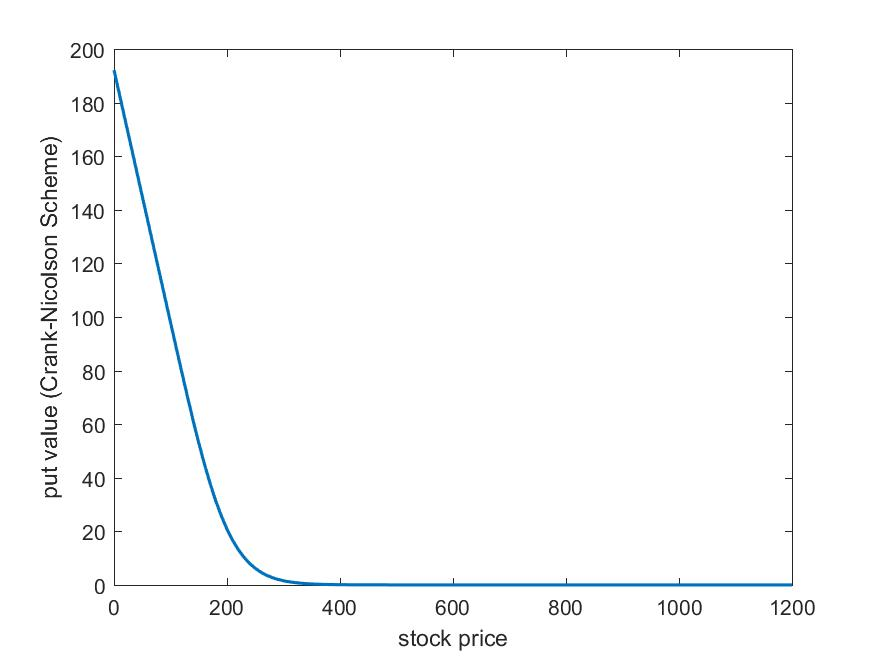
\includegraphics[width=8.5cm]{u0_CN.jpeg}
\subcaption*{Crank-Nicolson Scheme}
\end{subfigure}
\begin{subfigure}[c]{0.5\textwidth}
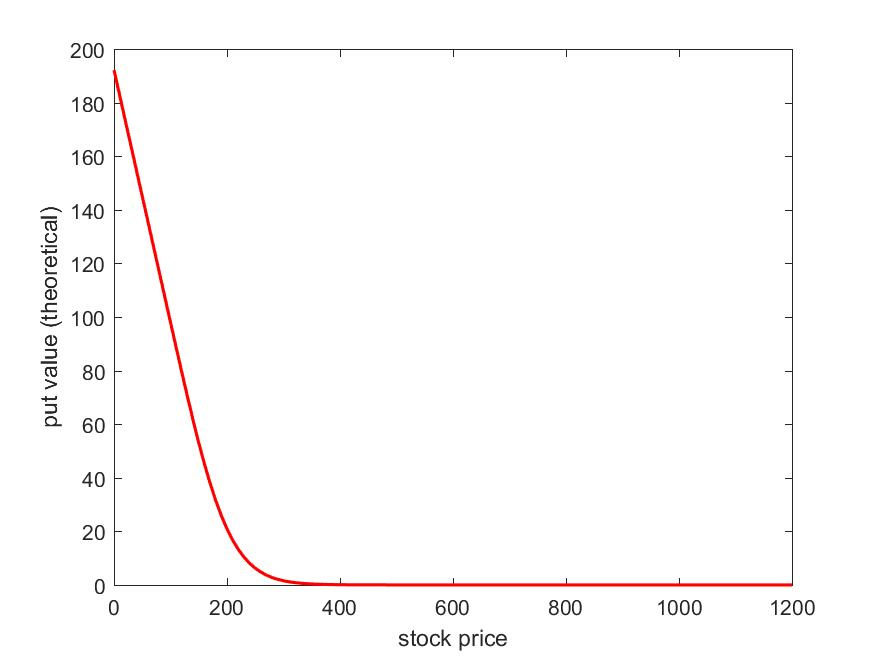
\includegraphics[width=8.5cm]{TheoEuroPut.jpeg}
\subcaption*{Theoretical}
\end{subfigure}
\caption{European Put value for different S: Crank-Nicolson Scheme vs. Theoretical}
\label{payoffPutCN}
\end{figure}
\begin{figure}[!h]
\centering
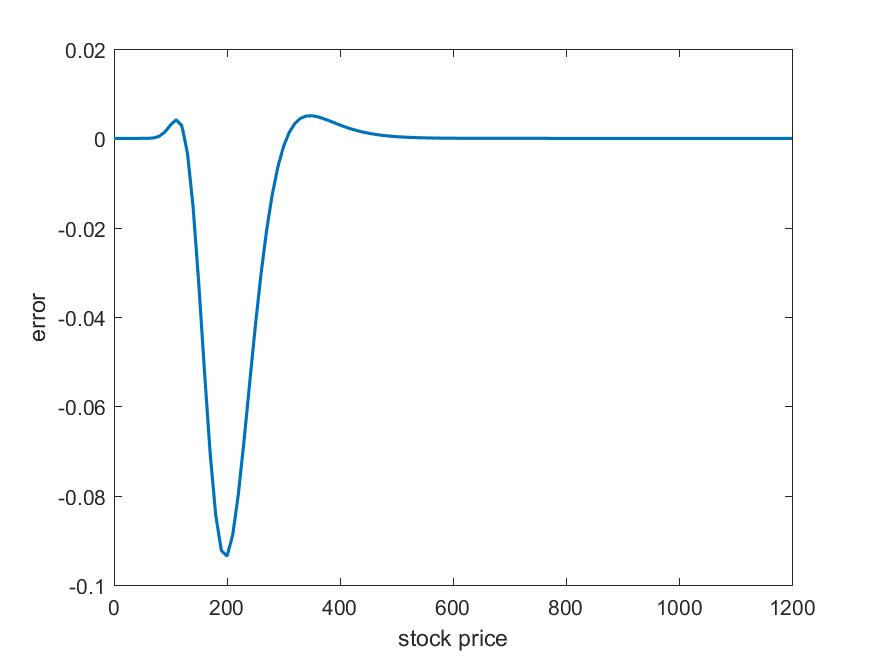
\includegraphics[width=10cm]{2D_CN.jpeg}
\caption{Crank-Nicolson Scheme - Error vs. Stock Price}
\label{2DErrorPutCN}
\end{figure}
\begin{figure}[h!]
\centering
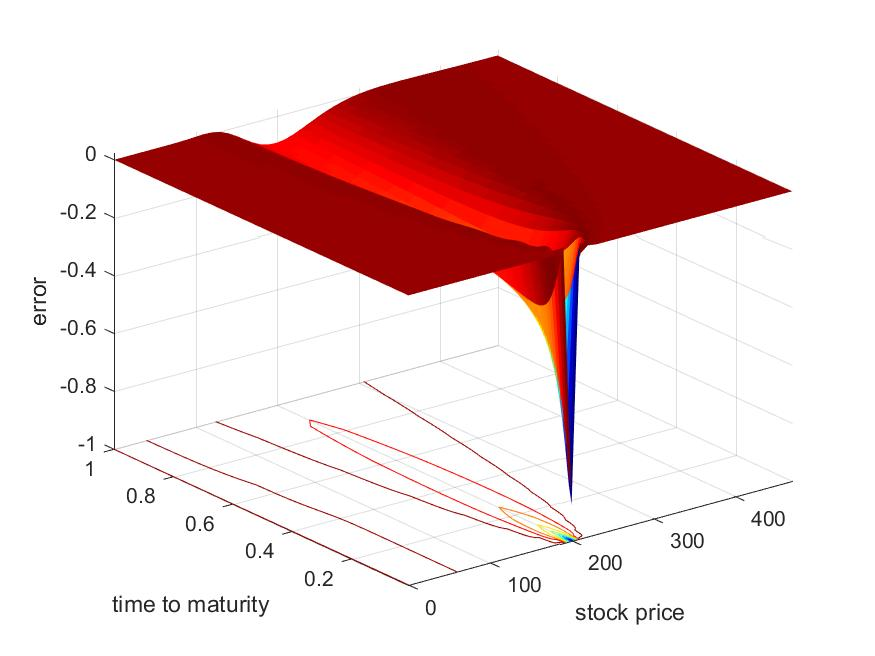
\includegraphics[width=10cm]{3D_CN.jpeg}
\caption{Crank-Nicolson Scheme - Error vs. Stock Price vs. Time to Maturity}
\label{3DErrorPutCN}
\end{figure}
Again it can clearly be seen that the CN scheme prices are almost identical to the theoretical price. For an underlying price of 200 the price of the European Put is 20.7951 (benchmark price = 20.8886). 
These errors in figure \ref{2DErrorPutCN} are similar to our former findings. The biggest deviation can be found when the option is  at-the-money due to the same reasons. In this case the error is 0.0936.  

Also the deviations decrease with increasing time steps as it can be seen in the 3D plot in \ref{3DErrorPutCN}. The maximum deviation which can be observed is 0.8762.

Comparing these results with the implicit scheme, one can see that the CN scheme computes more precise results.\footnote{Implicit Scheme 2D-Error: 0.1231 and 3D-Error: 0.9740.} This results are also in line with the theory because the truncation error of the CN scheme decreases,as it was  discussed in 3.2.2.,  with a speed $k^2$, instead of only $k$, as it was the case of the implicit scheme. This will be analysed in more detail in the last chapter of this paper.

\subsection{Technical Implementation}
The second part of the the main script \textit{$Task71\_73.m$} contains all necessary computations and plots for the Crank-Nicolson scheme. The script basically calls the function $CN.m$ which consists of the main algorithm for the Crank-Nicolson scheme.

The technical implementation is similar to the implicit scheme in the former chapter 2. The LR decomposition in this algorithm has to consider the B-Matrix on the right hand side. Furthermore other boundaries have to be implemented. 

As an output we get again the last \textit{u0\_CN} vector, as well as the errors for \textit{ERROR\_2D\_CN} for the 2D case and the \textit{ERROR\_3D\_CN} for the 3D case, as well as the maximum errors \textit{ME\_CN\_2D} and \textit{ME\_CN\_3D} for the 2D and 3D case, respectively.

\section{Richardson extrapolation method}
To improve accuracy we introduce an Richardson extrapolation method for the same fixed combination of M and N to the implicit and Crank-Nicholson scheme.\\
For the implicit scheme we use:
\begin{equation}
\dfrac{1}{3}(4U^{2N}_{4M}-U^N_M)
\label{REImp}
\end{equation}
For the Crank-Nicolson-Scheme we use:
\begin{equation}
\dfrac{1}{3}(4U^{2N}_{2M}-U^N_M)
\label{RECN}
\end{equation}
Following the same analysis as in the chapters, one can derive the truncation errors of the extrapolated functions. (Sturm, 2017):\\
For the extrapolated implicit scheme we get:
\begin{equation}
O(h^4+k^2)
\label{IMPTruncRE}
\end{equation}
and for the extrapolated Crank-Nicolson scheme:
\begin{equation}
O(h^4+k^2h^2+k^4)
\label{CNTruncRE}
\end{equation}

One can show that, the truncation error of the Crank-Nicolson scheme is of higher order and hence will deliver more precise results. 
\subsection{Discussion of Results}

\begin{figure}[!h]
\begin{subfigure}[c]{0.5\textwidth}
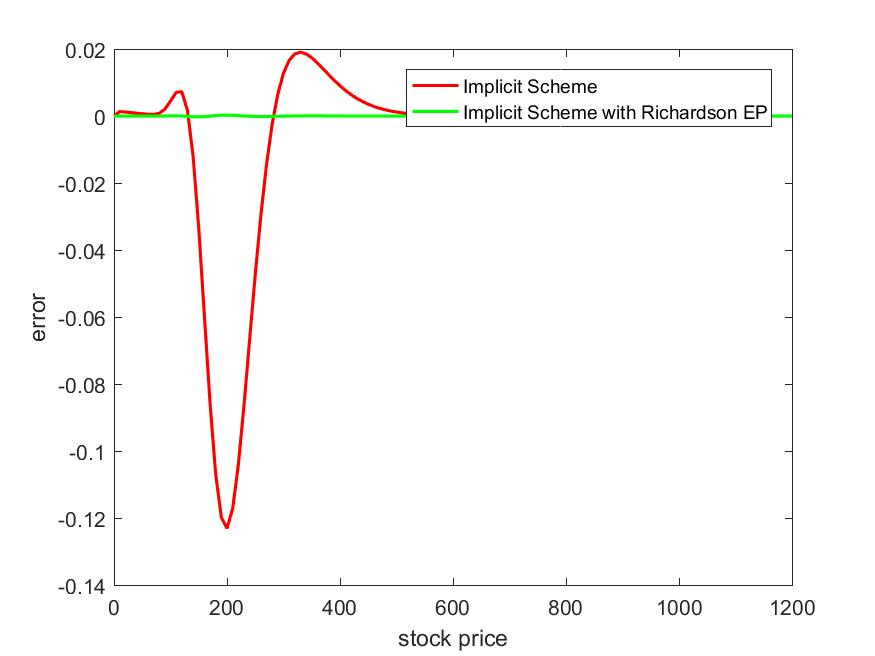
\includegraphics[width=8.5cm]{IMPvsRE.jpeg}
\subcaption*{Implicit Scheme}
\end{subfigure}
\begin{subfigure}[c]{0.5\textwidth}
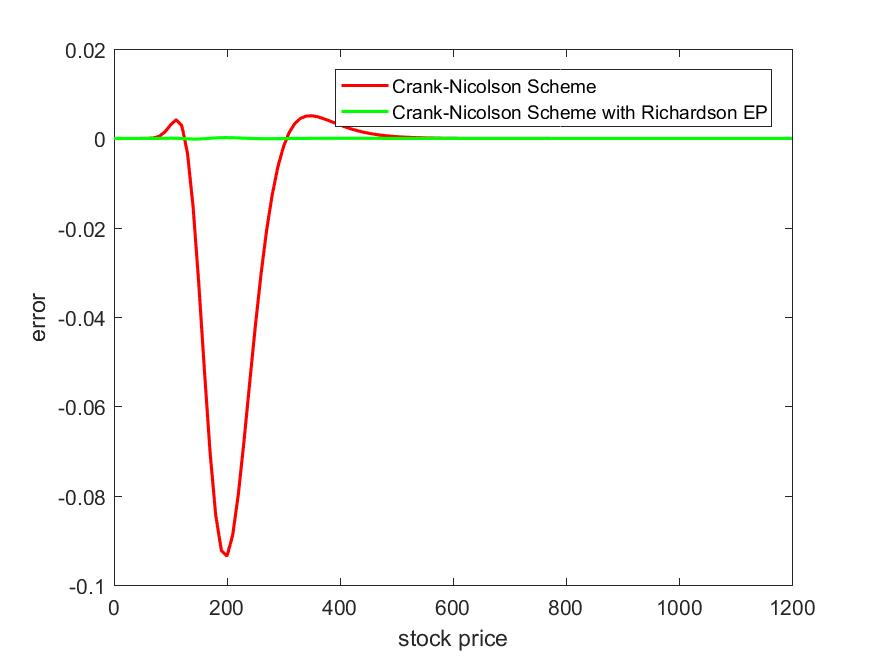
\includegraphics[width=8.5cm]{CNvsRE.jpeg}
\subcaption*{CN Scheme}
\end{subfigure}
\caption{2D-Errors - Standard Schemes vs. Extrapolation}
\label{2DvsRE}
\end{figure}
Figure \ref{2DvsRE} compares the standard implicit and Crank-Nicolson scheme methods with the extrapolated functions. The prices for the European Put at S=200 for the extended implicit and CN schemes are 20.8889 and 20.8888, respectively. As you can clearly see the methods decrease the errors significantly. The maximum errors of the extrapolated implicit and Crank-Nicolson cases are  2.6765e-04 (vs. 0.1231) and  1.7175e-04 (vs. 0.0936) respectively, which is a huge improvement compared to the calculation without extrapolation.
\begin{figure}[!h]
\begin{subfigure}[c]{0.5\textwidth}
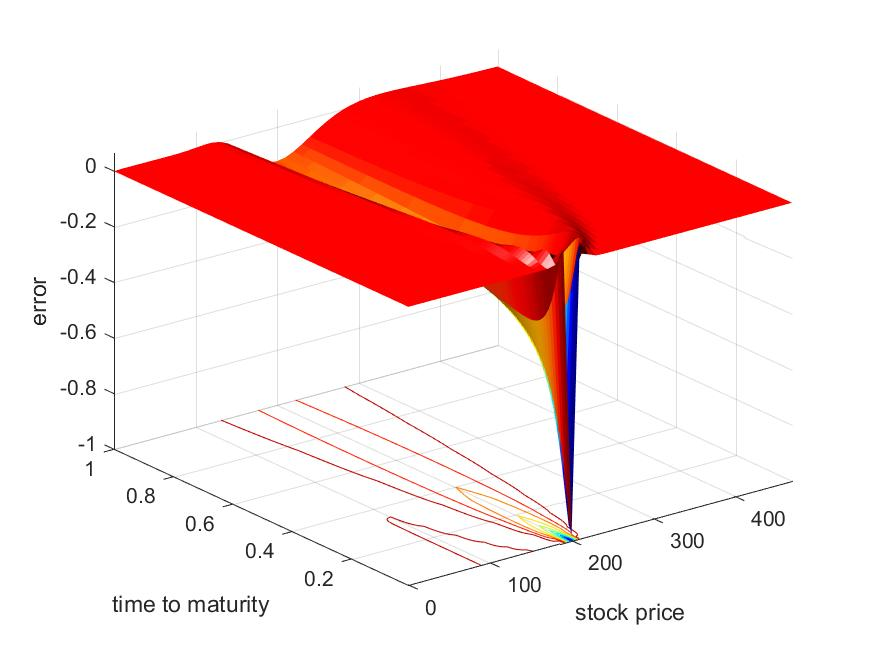
\includegraphics[width=8.5cm]{3D_Implicit.jpeg}
\subcaption*{Standard Implicit Scheme}
\end{subfigure}
\begin{subfigure}[c]{0.5\textwidth}
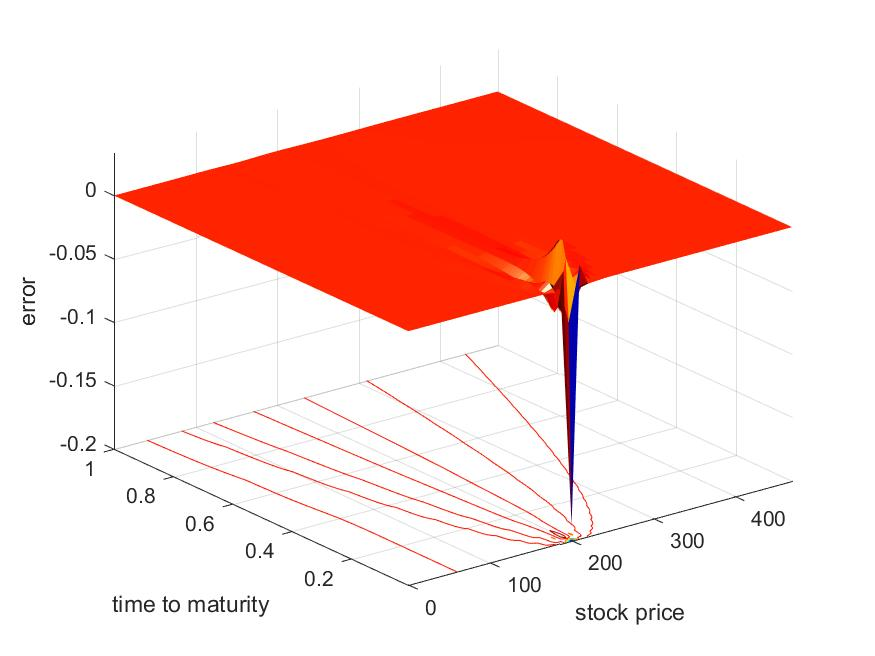
\includegraphics[width=8.5cm]{3D_IMPRE.jpeg}
\subcaption*{Implicit Scheme with Richardson Extrapolation}
\end{subfigure}
\caption{Standard Implicit Scheme vs. Extrapolation (3D-Errors)}
\label{3DCN1}
\end{figure}

\begin{figure}[!h]
\begin{subfigure}[c]{0.5\textwidth}
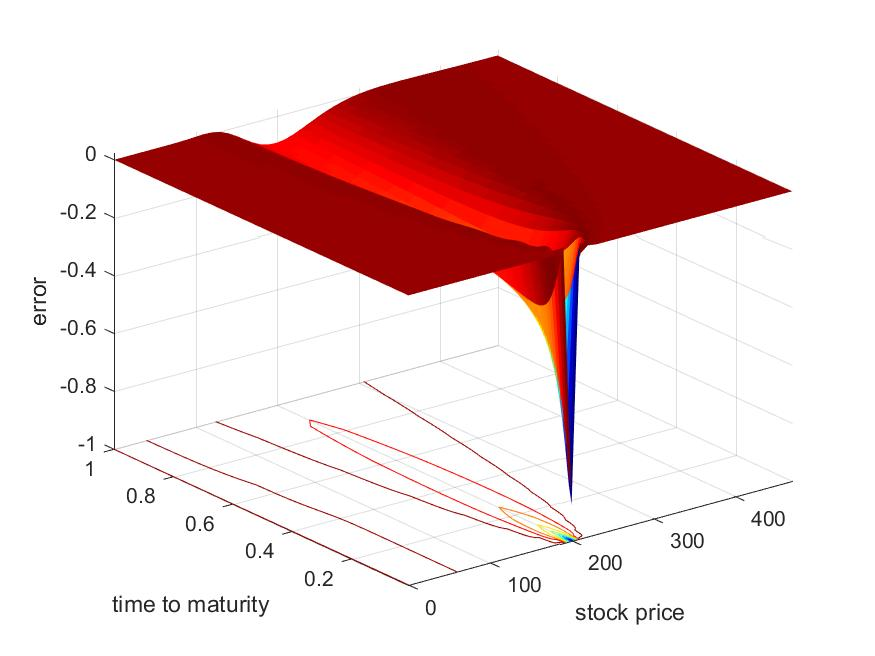
\includegraphics[width=8.5cm]{3D_CN.jpeg}
\subcaption*{Standard Implicit Scheme}
\end{subfigure}
\begin{subfigure}[c]{0.5\textwidth}
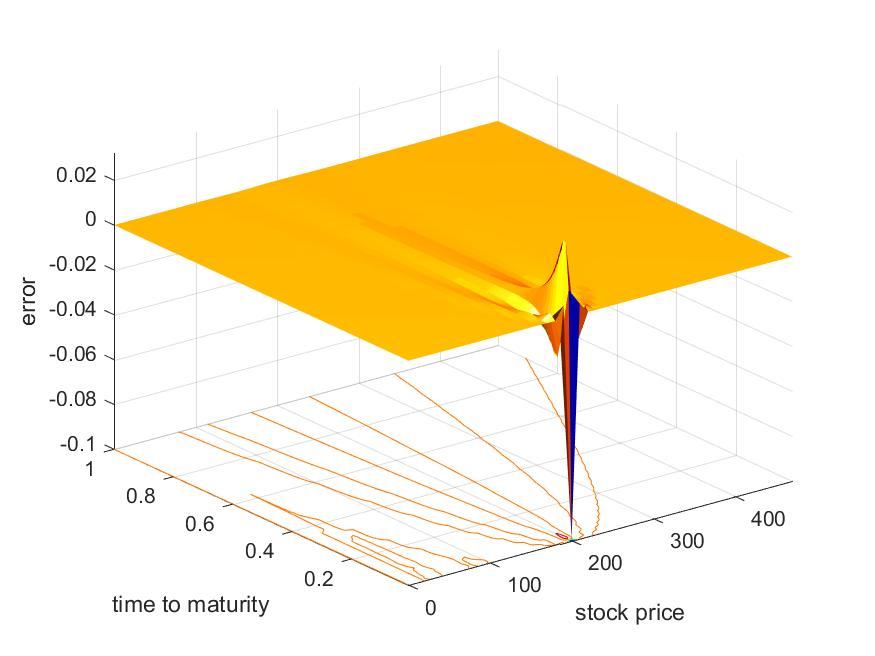
\includegraphics[width=8.5cm]{3D_CNRE.jpeg}
\subcaption*{Implicit Scheme with Richardson Extrapolation}
\end{subfigure}
\caption{Standard Crank-Nicolson Scheme vs. Extrapolation (3D-Errors)}
\label{3DCN2}
\end{figure}
Same holds for the 3D-error shown in figures \ref{3DCN1} and \ref{3DCN2}. Both extrapolation methods improves accuracy also for the 3D case as you can also observe in the maximum absolute error. In the 3D case the maximum absolute error of the extrapolated implicit and Crank-Nicolson schemes are 0.1881 (vs. 0.9740) and 0.0992 (vs. 0.8762).

The reason of this improvement can be explained by the truncation errors in (\ref{IMPTruncRE}) and (\ref{CNTruncRE}). The errors converge faster compared to the standard methods and hence deliver more precise results.

Note that higher accuracy comes with a higher computational effort. As you can see in equations (\ref{REImp}) and (\ref{RECN})  
bigger grids are necessary which can increase computational time significantly. This can be described as a trade off between accuracy and time, which will be discussed more in detail in chapter 5.
\subsection{Technical Implementation}
The third part of the the main script \textit{$Task71\_73.m$} contains all necessary computations and plots for the Richardson Extrapolation functions. The script calls the function \textit{$Implicit\_RE.m$} and \textit{$CN\_RE.m.$}
Each function basically calls the scheme functions \textit{Implicit.m} or \textit{CN.m} with respect to the grid-sizes defined by the Richardson extrapolation in Task 7.3. in the assignment. Since the Richardson extrapolation creates vectors of different sizes MxN, we have to cut the vector to the specific form (every 2nd row). The computations of the extrapolation are then just stored in an own \textit{u0 vector}.

To get the 3D-errors of the extrapolation, one has also to adjust the error matrices in order to fit. For the implicit scheme (4Nx2M) we only take every 4th column into account and cut every 2nd row away. For the CN scheme (2Mx2N) we only take every 2nd column into account and cut away every 2nd row.

As an output, we again get the \textit{u0} vectors, swell as the error vector (2D errors), matrix (3D errors) and its maximum absolute errors, for the implicit scheme and Crank-Nicolson scheme respectively.

\section{Efficiency Discussion: Accuracy and Computational Effort}
In this section we compare which method is the most efficient by computing the price of the European Put with the given parameters for increasing combinations of M and N. Therefore we fix the time dimension on the space dimension for M $\in [12:12:1200]$ in the following way.\\
For the first case:
\begin{equation*}
N=\dfrac{1}{72}M^2
\end{equation*}
For the second case:
\begin{equation*}
N=\dfrac{1}{1.2}M
\end{equation*}
\begin{figure}[!h]
\begin{subfigure}[c]{0.5\textwidth}
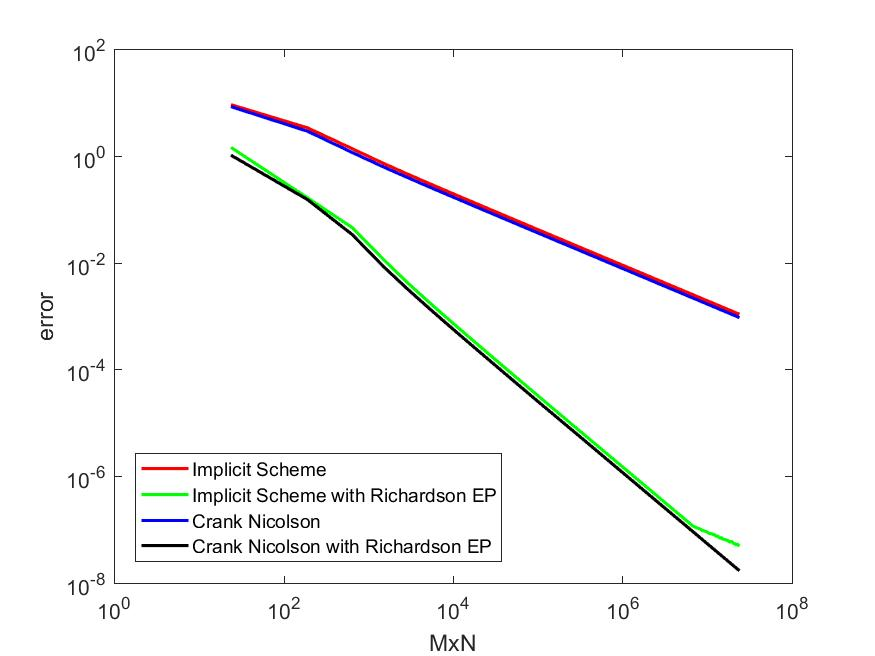
\includegraphics[width=8.5cm]{74_error.jpeg}
\subcaption*{$N=\dfrac{1}{72}M^2$}
\end{subfigure}
\begin{subfigure}[c]{0.5\textwidth}
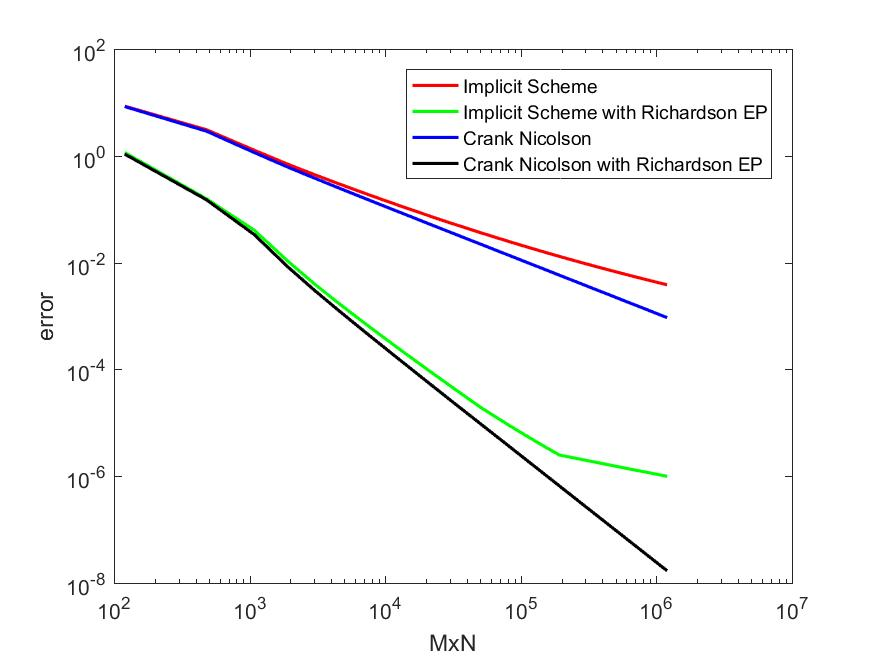
\includegraphics[width=8.5cm]{75_error.jpeg}
\subcaption*{$N=\dfrac{1}{1.2}M$}
\end{subfigure}
\caption{Errors Development for increasing step-sizes MxN (log-log-scale))}
\label{7ERROR}
\end{figure}
\begin{figure}[!h]
\begin{subfigure}[c]{0.5\textwidth}
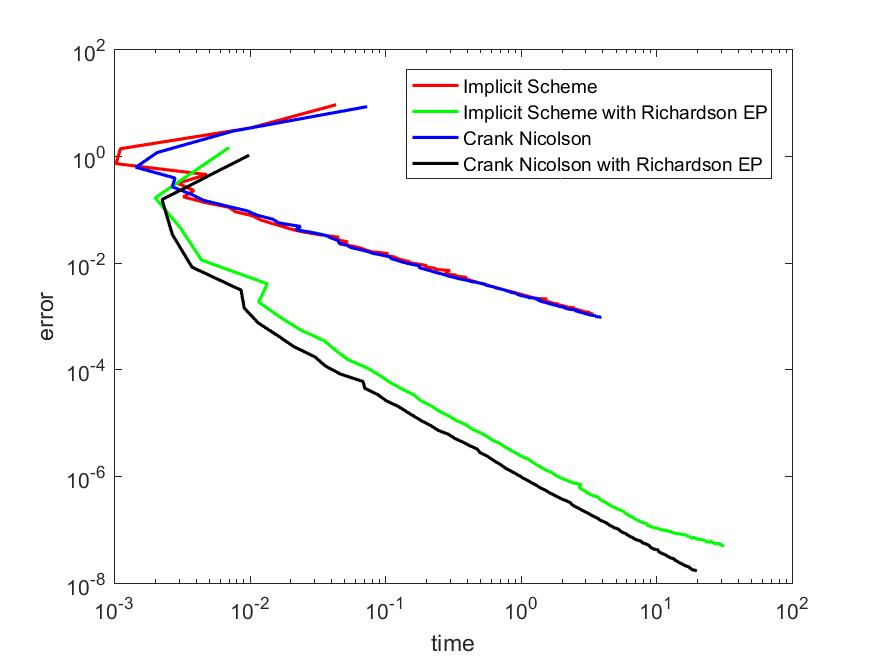
\includegraphics[width=8.5cm]{74_time.jpeg}
\subcaption*{$N=\dfrac{1}{72}M^2$}
\end{subfigure}
\begin{subfigure}[c]{0.5\textwidth}
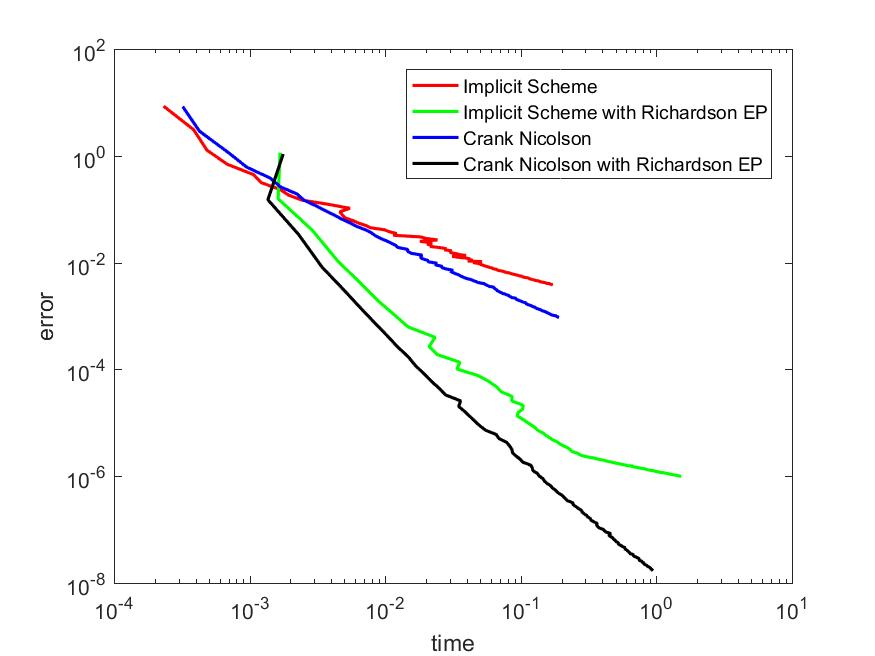
\includegraphics[width=8.5cm]{75_time.jpeg}
\subcaption*{$N=\dfrac{1}{1.2}M$}
\end{subfigure}
\caption{Trade-Off: Computational Time vs. Error}
\label{7TIME}
\end{figure}

In figure \ref{7ERROR} one can see that the error decreases with increasing MxN combinations and the Crank-Nicolson scheme delivers, due to the smaller truncation error, a more precise approximation then the implicit scheme. 

Also one can easily observe that the Richardson extrapolation of the schemes clearly improves accuracy. It is also noticeable that in the extrapolated case, the CN function dominates the implicit function, even tough it uses fewer grid points to extrapolate (CN uses 2Nx2M while the implicit scheme uses 2Nx4M grid points). Again, this is in line with the theory. As we have shown the truncation errors of the extrapolated functions are of higher order compared to the case without extrapolation. Also the truncation errors of the CN scheme in the extrapolated case are of higher order compared to the implicit case.

Plot \ref{7TIME} illustrates the trade off between computational time and accuracy.\footnote{Note that time plots might differ from run to run of the function.} One can see that for a decreasing error size the extrapolated functions are more efficient. Hence, for our programmed algorithm, the extrapolated CN function, delivers the most efficient results for relatively big grid sizes MxN. But this, in fact, also implies that efficiency is depended on the size of grid. For small grids it may makes sense to dispense with extrapolation as you can see in figure \ref{7TIME1}.

\begin{figure}[!h]
\begin{subfigure}[c]{0.5\textwidth}
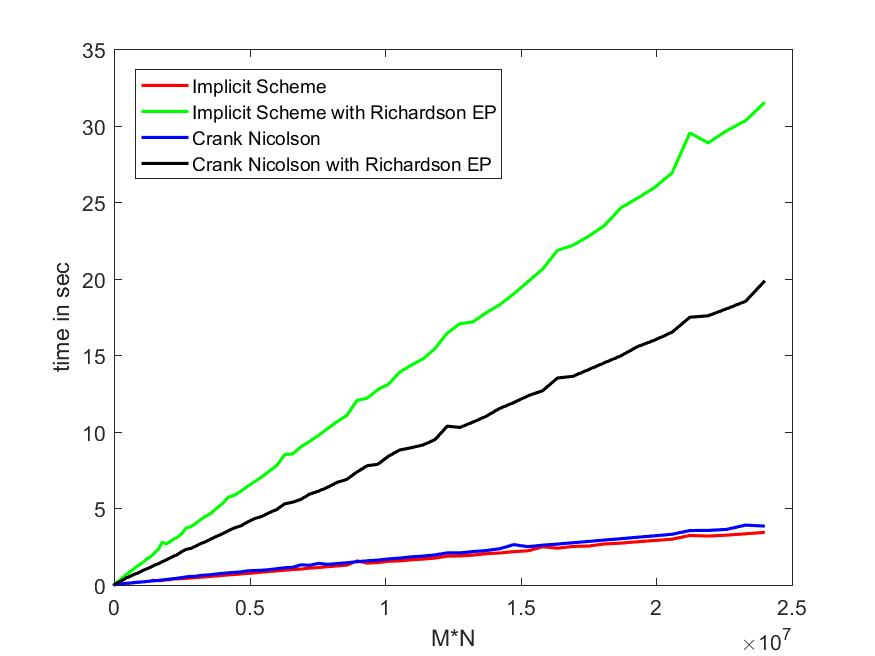
\includegraphics[width=8.5cm]{74_time2.jpeg}
\subcaption*{$N=\dfrac{1}{72}M^2$}
\end{subfigure}
\begin{subfigure}[c]{0.5\textwidth}
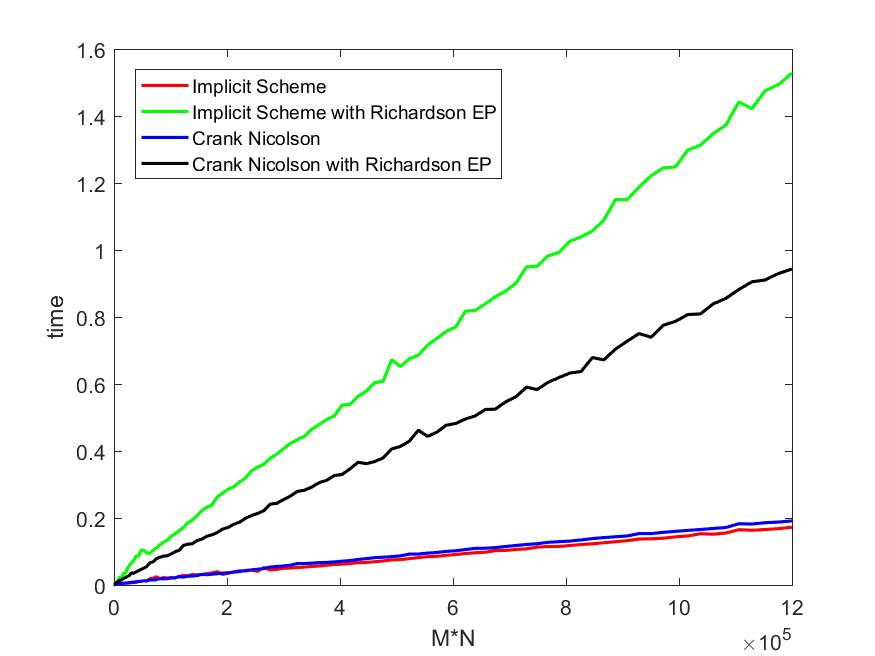
\includegraphics[width=8.5cm]{75_time2.jpeg}
\subcaption*{$N=\dfrac{1}{1.2}M$}
\end{subfigure}
\caption{Errors Development for increasing step-sizes MxN (log-log-scale))}
\label{7TIME1}
\end{figure}

Comparing the left and right figures of illustrations \ref{7ERROR}, \ref{7TIME} and \ref{7TIME1} makes clear that an increase in the grid-size does not necessary increase accuracy, especially when it comes to efficiency regarding computational effort. 
In particular, this can be seen in figure \ref{7TIME1}. A strong increase in the grid size may come with an increase in precision but again with an large increase in computational time and inefficient computations. 

Taking everything together, when it comes to the trade off between accuracy and computational effort, the Crank-Nicolson scheme delivers not only the most accurate  but also the most efficient results with respect to computational time. Hence the Crank-Nicolson scheme should always be preferred to the implicit method, especially for modified Richardson extrapolation functions. 
\subsection{Technical Implementation}
Task 7.4 and 7.5 can be solved by running the scripts \textit{$Task74.m$} and \textit{$Task75.m$}. In these scripts we constructed for each of the four methods a for-loop, where the function is called with respect to the computational 2D-error, for each specific MxN combination. Since we are interested in the computational time we additionally count the time by including the command 'tic' and 'toc' into each for-loop. Note that due to system performance, the time measurement might differ slightly from run to run. The output vectors are later plotted with a \textit{loglog}-command to get a log-scale on the x and y axis. 

Note that all computations were run on an Windows 10 64-bit operation system with an Intel(R) Core(TM) i7-5500U CPU \@ 2.40 Ghz. Since the computation might take several minutes, the data of task 7.4. and 7.5. in \textit{74\_Errors.mat} and \textit{75\_Errors.mat} were additionally added.
\newpage
\section{References}

Brandimarte, Paolo. \textit{Numerical Methods in Finance and Economics - A MATLAB-Based Introduction}, $2^{nd}$ ed., John Wiley \& Sons, Hoboken NJ, 2006.\\

Fusai, Gianluca and Roncoroni, Andrea. \textit{Implementing Models in Quantitative Finance: Methods and Cases.} Springer-Verlag, Berlin Heidelberg New York 2008.\\

Hirsa, Ali. \textit{Computational Methods in Finance}. Chapman \& Hall/ CRC Press, Boca Raton FL, 2013.\\

Sturm, Pascal. \textit{Assignment \#2: Implicit Finite Difference Methods}. Numerical Methods in Finance Assignments, T\"ubingen, 2017.
\end{document}

